\usepackage{amsmath}
\usepackage{amssymb}
\usepackage[%
    isbn=false,
]{biblatex}
\usepackage{etoolbox}
\usepackage{lstautogobble}
\usepackage{pgffor}
\usepackage{siunitx}
\usepackage{tabularray}
\UseTblrLibrary{booktabs,siunitx}
\usepackage[listings,skins,theorems,xparse]{tcolorbox}
\usepackage{tikz}
\usetikzlibrary{calc}
\usetheme[miniframes-enhanced,framenumber-footline]{Mumbai} % available at https://github.com/vachan-potluri/beamer_themes/tree/main/Mumbai



\DeclareTotalTCBox{\inlinecode}{m}{%
    verbatim,
    size=tight,
    boxsep=2pt,
    arc=0pt,
    bottomrule=0pt,
    toprule=0pt,
    leftrule=0pt,
    rightrule=0pt,
}{\lstinline|#1|} % for printing inline code
\colorlet{ScilabComment}{green!50!black}
\lstdefinestyle{ScilabStyle}{%
    % scilab formatting style
    language=Scilab,
    backgroundcolor=\color{gray!10},
    basicstyle=\linespread{1.25}\ttfamily\small,
    commentstyle=\color{ScilabComment},
    keywordstyle=\bfseries\color{blue},
    numberstyle=\color{gray}\sffamily\footnotesize,
    stringstyle=\color{red},
    basewidth=0.5em,
    breakatwhitespace=false,
    breaklines=true,
    postbreak=\hbox{$\hookrightarrow$},
    captionpos=t,
    frame=l,
    keepspaces=true,
    numbers=none,
    numbersep=5pt,
    showspaces=false,
    showstringspaces=false,
    showtabs=false,
    tabsize=2,
    morekeywords=[2]{\%t,\%f,\%pi,\%e,\%i,\%inf,\%nan,\%eps},
    keywordstyle=[2]\color{magenta},
    morecomment=[s][\bfseries\color{orange}]{/*}{*/},
    %morecomment=[l][\itshape\color{blue!30!green}]{//-},
    autogobble=true,
    xleftmargin=0.25em,
    %xrightmargin=1em,
}
\lstset{style=ScilabStyle}
\newcommand{\email}[1]{\href{mailto:#1}{\texttt{#1}}} % for email ids
\newcommand{\hint}[1]{{\small\alert{Hint: #1}}}
\newcommand{\keyword}[1]{#1}
\newcommand{\matlab}{\texttt{MATLAB}}
\newcommand{\scilab}{\texttt{Scilab}}
\newcommand{\scinotes}{\texttt{SciNotes}}
\newcommand{\setitemsep}[1]{\setlength\itemsep{#1}}
\newtcbox{\key}{%
    enhanced,
    on line,
    colback=gray!25,
    size=fbox,
    bottomrule=0pt,
    toprule=0pt,
    leftrule=0pt,
    rightrule=0pt,
    fontupper=\ttfamily,
    drop fuzzy shadow,
} % for printing keyboard keys
\newtcolorbox{exercise}{%
    code={
        \usebeamercolor{block title}
        \colorlet{titlebg}{bg}
        \colorlet{titlefg}{fg}
        \usebeamercolor{block body}
        \colorlet{bodybg}{bg}
        \colorlet{bodyfg}{fg}
    },
    colbacktitle=titlebg,
    coltitle=titlefg,
    colback=bodybg,
    coltext=bodyfg,
    size=fbox,
    title={Exercise},
}% boxed env for exercises




\addbibresource{references.bib}



\begin{document}

\setlength\leftmargini{1em} % left margin, first level itemize
\setlength\leftmarginii{\leftmargini} % left margin, 2nd level
\setlength\leftmarginiii{\leftmarginii} % left margin, 3rd level

{
    \setbeamertemplate{headline}{}
    \setbeamertemplate{footline}{}
    \title{Scilab}
    \author[Vachan Potluri]{%
        Vachan Potluri\\
        \email{vachanpotluri@iitb.ac.in}
    }
    \date{Spring 2023}
    \begin{frame}
        \titlepage
    \end{frame}
}

\begin{frame}{Introduction}
    \begin{block}{What is \scilab?}
        A free alternative to \matlab
    \end{block}
    \begin{block}<visible@2->{What can it do?}
        \begin{enumerate}
            \item Advanced calculator
            \item Programming
            \item Plotting, visualisation
        \end{enumerate}
    \end{block}
\end{frame}

\section{Basics}
\subsection{As a calculator}
\begin{frame}[fragile]{Simple calculations}
    Try out these and see if they give expected results
    \begin{lstlisting}[numbers=left]
        2+3-4
        4^2
        4**4
        6/4
        2+(2^2-(1/2))
        1e-3 + 1d-2
    \end{lstlisting}
\onslide<2->
    See what happens when you add a semicolon
    \begin{lstlisting}
        6/4;
    \end{lstlisting}
\end{frame}

\begin{frame}[fragile]{Variables}
    All calculations are stored by default in \inlinecode{ans}
    \begin{lstlisting}
        6/4;
        ans
    \end{lstlisting}
\onslide<2->
    You can specify a variable to store the value instead
    \begin{lstlisting}
        pi_approx = 22/7;
    \end{lstlisting}
    And see its value later
    \begin{lstlisting}
        pi_approx
        disp(pi_approx)
    \end{lstlisting}
\end{frame}

\begin{frame}[fragile]{More on variables}
    Some useful pre-defined variables
    \begin{lstlisting}[numbers=left]
        %pi
        %e
        %i
        %t
        %f
        %inf
        %nan
        %eps
    \end{lstlisting}
\end{frame}

\begin{frame}[fragile]{Pre-defined functions}
    See if the outputs of these lines are as expected
    \begin{lstlisting}[numbers=left]
        abs(-2)
        min(3,4,5)
        max(-2,-3,-4)
        sin(%pi/2)
        cos(%pi)
        tan(%pi/4)
        asin(1)/(%pi/2)
        exp(2)/%e^2
        log10(100)
        log(%e)
    \end{lstlisting}
    Auto-completion: hit \key{TAB}
\end{frame}

\begin{frame}[fragile]{Other \scilab{} windows}
\begin{itemize}
    \item \keyword{Variable Browser}
    \begin{itemize}
        \item Only lists user-defined variables
        \item To list all variables:
        \begin{lstlisting}
            whos
        \end{lstlisting}
        \onslide<2->
        \item You can delete all or specific user-defined variables
        \begin{lstlisting}
            pi_approx = 22/7;
            disp(pi_approx)
            clear pi_approx
            disp(pi_approx)
        \end{lstlisting}
    \end{itemize}
    \onslide<3->
    \item \keyword{Command History}
    \begin{itemize}
        \item Execute an old command by double clicking
        \item Can also navigate using $\uparrow$ and $\downarrow$ keys
        \item Clear screen using \inlinecode{clc}
    \end{itemize}
    \onslide<4->
    \item \keyword{File Browser}
    \begin{itemize}
        \item Useful when working with multiple files
    \end{itemize}
\end{itemize}
\end{frame}

\subsection{Arrays and matrices}
\begin{frame}[fragile]{Basic matrix creation}
    Wrap inside \inlinecode{[]}, use \inlinecode{,} and \inlinecode{;} to separate columns and rows
    \begin{lstlisting}
        x = [1,2,3]
        y = [4;5;6;7]
        A = [1,0;0,1]
    \end{lstlisting}
\onslide<2->
    \scilab{} will warn you if the dimensions are inconsistent
    \begin{lstlisting}
        B = [1,2,3;4,5]
    \end{lstlisting}
\onslide<3->
    Adding \inlinecode{'} will transpose the matrix
    \begin{lstlisting}
        B = [1,2,3;4,5,6];
        B'
    \end{lstlisting}
\onslide<4->
    You can fill matrices with pre-existing matrices
    \begin{lstlisting}
        row1 = [1,2,3,4];
        row2 = [5,6,7,8];
        M = [row1;row2]
    \end{lstlisting}
\end{frame}

\begin{frame}[fragile]{Special functions for matrix creation}
    Creating ranges
    \begin{lstlisting}
        i = 1:10
        j = 1:2:10
        x = 0:0.1:1
        y = linspace(0,1,25)
    \end{lstlisting}
\onslide<2->
    Some useful commands for creating dummy matrices of required size
    \begin{lstlisting}
        A = zeros(2,2)
        B = ones(3,2)
        M = eye(3,3)
    \end{lstlisting}
\onslide<3->
    Can you make sense of this result?
    \begin{lstlisting}
        M = [[zeros(1,2);ones(1,2);eye(2,2)],ones(4,1)]
    \end{lstlisting}
\end{frame}

\begin{frame}[fragile]{Matrix operations}
    \begin{columns}
        \begin{column}{0.49\linewidth}
            Scalar operations affect all elements of matrices
            \begin{lstlisting}
                A = eye(3,3);
                A*2
                A/4
                A+5
            \end{lstlisting}
\onslide<2->
            \scilab{} automatically figures out matrix operations too
            \begin{lstlisting}
                B = 2*ones(3,3)
                A+B
                A*B
                B^2
            \end{lstlisting}
        \end{column}
        \begin{column}{0.49\linewidth}
\onslide<3->
            Special element wise operations
            \begin{lstlisting}
                A.*B
                A.^B
                A./B
                A.^2
            \end{lstlisting}
            How is \inlinecode{A^2} different from \inlinecode{A.^2}?
        \end{column}
    \end{columns}
\end{frame}

\begin{frame}[fragile]{Matrix functions}
    Most \scilab{} functions can operate element-wise on matrices
    \begin{lstlisting}
        A = %pi/2*[0,1;2,3];
        sin(A)
    \end{lstlisting}
\onslide<2->
    Some special functions for matrices
    \begin{lstlisting}
        length(A)
        size(A)
        sum(A)
        det(A)
        inv(A)
        trace(A)
    \end{lstlisting}
\end{frame}

\begin{frame}[fragile]{Matrix indexing}
    \begin{columns}
        \begin{column}{0.49\linewidth}
            Access elements using \inlinecode{(row,col)}
            \begin{lstlisting}
                A = eye(3,3);
                A(1,2) = 2;
                A
            \end{lstlisting}
\onslide<2->
            A single index can also be used: increments column-wise
            \begin{lstlisting}
                A(4)
            \end{lstlisting}
\onslide<3->
            Extract rows and columns using \inlinecode{:}
            \begin{lstlisting}
                A(:,2)
                A(1,:)
            \end{lstlisting}
\onslide<4->
            Special symbol \inlinecode{\$}
            \begin{lstlisting}
                A($,3)
            \end{lstlisting}
        \end{column}
        \begin{column}{0.49\linewidth}
\onslide<5->
            Arrays can also be used to access and modify
            \begin{lstlisting}
                A([1,2],2)
                A(4,:) = [10,20,30]
            \end{lstlisting}
\onslide<6->
            See if this makes sense
            \begin{lstlisting}
                A = eye(4,4);
                j = [2,4];
                A(1,j) = j
                A([7,8]) = 50
                A($,$) = -1
                B = [9,10;j];
                A(B) = 100
            \end{lstlisting}
        \end{column}
    \end{columns}
\end{frame}

\subsection{Miscellaneous}
\begin{frame}[fragile]{Strings}
    Wrap in \inlinecode{""} or \inlinecode{''}
    \begin{lstlisting}
        fname = "Vachan";
        lname = 'Potluri';
        fname + lname
    \end{lstlisting}
\onslide<2->
    Function \inlinecode{string} converts variables to strings
    \begin{lstlisting}
        A = eye(2,2)
        string(A)
    \end{lstlisting}
\end{frame}

\begin{frame}[fragile]{Saving and loading data}
    \scilab{} has a working directory
    \begin{lstlisting}
        pwd
    \end{lstlisting}
    Working directory can be changed from File Browser (and also using \inlinecode{cd} or \inlinecode{chdir})\\[0.5em]
\onslide<2->
    Function \inlinecode{save} saves user-defined variables to a file in working directory
    \begin{lstlisting}
        x = 1.5;
        A = [1,2;3,4]
        save("data.dat")
    \end{lstlisting}
\onslide<3->
    These variables can be loaded for use later
    \begin{lstlisting}
        listvarinfile("data.dat")
        load("data.dat")
    \end{lstlisting}
\end{frame}

\begin{frame}[fragile]{Accessing help}
    \scilab's built-in help functionality is very useful
    \begin{lstlisting}
        help
        help save
    \end{lstlisting}
\end{frame}

{
% modify ',' to allow math mode line break at ','
% https://tex.stackexchange.com/a/67540/133968
\def\OldComma{,}
\catcode`\,=13
\def,{%
    \ifmmode%
    \OldComma\discretionary{}{}{}%
    \else%
    \OldComma%
    \fi%
}%
\sisetup{list-separator={,~}}
\begin{frame}{Exercises\footfullcite{amos2017}}
    \begin{columns}
        \begin{column}{0.49\linewidth}
            \begin{exercise}
                The pressure drop $\Delta p$ required for a flow rate $Q$ in a pipe of diameter $D$ is
                \begin{equation*}
                    \Delta p = 4.52 \frac{Q^{1.85}}{C^{1.7} D^{4.87}}
                \end{equation*}
                Find $\Delta p$ for these combinations of flow rates and diameters:
                \begin{itemize}
                    \item $Q=\numlist{50;100;200;400;1000}$
                    \item $D=\numlist{0.5;1;1;2;4}$
                \end{itemize}
                Use $C=2.5$ for all cases
            \end{exercise}
        \end{column}
        \begin{column}{0.49\linewidth}
\onslide<2->
            \begin{exercise}
                A magic square is a matrix in which all rows, columns and diagonals sum to same number.
                \begin{enumerate}
                    \item Generate a magic square of size 10
                    \item Verify that all rows and columns sum up to the same value
                \end{enumerate}
                \hint{search \scilab{} help for the function \inlinecode{testmatrix}, and use the \inlinecode{sum} function}
            \end{exercise}
        \end{column}
    \end{columns}
\end{frame}
}

\section{Programming}
\subsection{Getting familiar with script files}
\begin{frame}[fragile]{\scinotes: built-in editor}
    \begin{itemize}
        \setitemsep{1em}
        \item Console is only useful for short calculations
        \begin{itemize}
            \item Imagine typing 10s of commands again after changing just one input
        \end{itemize}
        \item<2-> A single file containing all commands is useful for large calculations
        \item<3-> Such files are called ``scripts'' or ``executables''
        \item<4-> \scinotes{} is \scilab's built-in GUI for handling scripts
        \item<5-> Customary to save such files with \inlinecode{.sce} or \inlinecode{.sci} extension
        \item<6-> Comments begin with \inlinecode{//}, or can be wrapped with \inlinecode{/* */}
        \begin{lstlisting}
            // this is a single line comment
            /* this is a
               multi-line comment */
        \end{lstlisting}
    \end{itemize}
\end{frame}

\begin{frame}[fragile]{Conditional statements}
    Can you make sense of this?
    \begin{lstlisting}
        x=6;
        reminder = modulo(x,3);
        
        if reminder==0 then
            disp("3 divides x")
        elseif reminder==1 then
            disp("x leaves reminder 1 when divided by 3")
        else
            disp("x leaves reminder 2 when divided by 3")
        end
    \end{lstlisting}
    \hint{look at help for function \inlinecode{modulo}}\\[1em]
\onslide<2->
    Logical expressions generally use \inlinecode{==, ~=, <, <=, >, >=, &&, \|\|, \%t, \%f}
\end{frame}

\begin{frame}[fragile]{Loops}
    \begin{columns}
        \begin{column}{0.5\linewidth}
            \begin{lstlisting}
                array = 1:10;
                value = 5;
                
                for a=array
                    if value==a then
                        disp("Value exists in array");
                        break;
                    end
                end
            \end{lstlisting}
            What does \inlinecode{break} statement do?
        \end{column}
        \begin{column}{0.49\linewidth}
            \onslide<2->
            \scilab{} always loops over columns
\onslide<3->
            \begin{lstlisting}
                array=[1;2;3]
                i=1;
                for a=array
                    disp("Element " + string(i) + ":")
                    disp(a)
                    i = i+1;
                end
            \end{lstlisting}
        \end{column}
    \end{columns}
\end{frame}

\begin{frame}[fragile]{Functions}
    \begin{lstlisting}
        function [Tf,Tk] = centigradeToFarenhietKelvin(Tc)
            Tf = Tc*9/5 + 32;
            Tk = Tc + 273;
        endfunction
        
        [Tf,Tk] = centigradeToFarenhietKelvin(37);
        disp(Tf)
        disp(Tk)
    \end{lstlisting}
    Here \inlinecode{Tf} and \inlinecode{Tk} are the ``return'' values; \inlinecode{Tc} is the parameter\\[0.5em]
\onslide<2->
    Can also have multiple parameters
    \begin{lstlisting}
        function s = sum(a,b)
            s = a+b;
        endfunction
        disp(sum(1,2));
    \end{lstlisting}
\end{frame}

\begin{frame}[fragile]{Exercises}
    \small
    \vspace{-1em}
    \begin{exercise}
        Write a function to calculate the cross product of two 3d vectors
        \begin{lstlisting}
            function v = cross_product(v1,v2)
                // fill this
            endfunction
        \end{lstlisting}
    \end{exercise}
\onslide<2->
    \begin{exercise}
        Write a function that takes in an array and a value, and returns the indices where the value occurs in an array.\\
        Example: for \inlinecode{array=[1,2,1,4,5,2]} and \inlinecode{value=2}, the function should return \inlinecode{[2,6]} (since \inlinecode{array(2)=array(6)=value})
        \begin{lstlisting}
            function indices = multiple_find(array,value)
                // fill this
            endfunction
        \end{lstlisting}
    \end{exercise}
\end{frame}

\subsection{Multiple file projects}
\begin{frame}[fragile]{Working with multiple files}
    \begin{itemize}
        \setitemsep{1em}
        \item Many times we use multiple user-written functions to accomplish our task
        \item<2-> Having them all in a single file makes it hard to read and debug
        \item<3-> Splitting the script into multiple files is preferable
        \begin{itemize}
            \item One for each function
            \item One main file
        \end{itemize}
        \item<4-> How to access content from another file?
    \end{itemize}
    \begin{columns}
        \begin{column}{0.5\linewidth}
\onslide<4->
            \begin{lstlisting}[title={\small \inlinecode{my\_function\_file.sce}}]
                function y=my_function(x)
                    // do something
                endfunction
            \end{lstlisting}
        \end{column}
        \begin{column}{0.5\linewidth}
\onslide<5->
            \begin{lstlisting}[title={\small \inlinecode{main.sce}}]
                // 'include' the file
                exec("my_function_file.sce",-1);
                // use the function
                result=my_function(2.5);
            \end{lstlisting}
        \end{column}
    \end{columns}
\end{frame}

\begin{frame}[fragile]{Exercises}
    \begin{exercise}
        \begin{enumerate}
            \setitemsep{1em}
            \item Recall the \inlinecode{cross_product()} function you have written previously. Save it in a file \inlinecode{cross_product.sce}
            \item<2-> Write a file \inlinecode{vector_norm.sce} which contains a function \inlinecode{vector_norm()} to calculate the length (norm) of a 3d vector
            \item<3-> Now in the file \inlinecode{triangle_area.sce}, write a function to calculate the area of an arbitrarily oriented triangle with points $p_1$, $p_2$ and $p_3$
            \begin{lstlisting}
                function area = triangle_area(p1, p2, p3)
                    // fill this
                endfunction
            \end{lstlisting}
            \hint{The area of a triangle is half the magnitude of cross product of any of its two sides}
        \end{enumerate}
    \end{exercise}
\end{frame}

\begin{frame}[fragile]
    \begin{exercise}
        We will calculate $\pi$ approximately here
        \begin{enumerate}
            \item Write a function \inlinecode{get_random_point()} which generates a random point in a 2d square $x \in [0,1],\ y \in [0,1]$\\
            \hint{Use the \inlinecode{rand} function of \scilab}
            \item<2-> Now write a function \inlinecode{inside_circle()} which takes any point and returns a boolean value saying whether or not the point lies inside the unit circle $x^2+y^2=1$
            \item<3-> Now write a function \inlinecode{approximate_pi()} that takes $N$ is an parameter and does the following
            \begin{itemize}
                \item Generate $N$ random points
                \item Find out how many of these points (say $N_i$) lie inside the unit circle
                \item Return the value $N_i/N$
            \end{itemize}
        \end{enumerate}
\onslide<3->
        \begin{columns}
            \begin{column}{0.5\linewidth}
                \begin{equation*}
                    \frac{N_i}{N} \to \frac{\pi}{4}\ \text{as}\ N \to \infty
                \end{equation*}
            \end{column}
            \begin{column}{0.5\linewidth}
                \begin{figure}
                    \centering
                    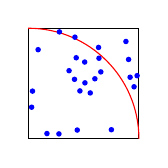
\begin{tikzpicture}[x=4em,y=4em]
                        \draw (0,0) rectangle (1,1);
                        \draw [red] (1,0) arc[start angle=0, end angle=90, radius=1];
                        \foreach \n in {1,2,...,25} {%
                            % add random points in the unit square
                            \fill[blue] (rand*0.5+0.5,rand*0.5+0.5) circle[radius=1pt];
                        }
                    \end{tikzpicture}
                \end{figure}
            \end{column}
        \end{columns}
        This is known as the Monte-Carlo simulation
    \end{exercise}
\end{frame}

\section{Plotting}

\subsection{Introduction}
\begin{frame}{A useful feature: plotting ability}
    \begin{itemize}
        \setitemsep{1em}
        \item Many basic programming languages do not have inbuilt plotting ability
        \item<2-> Results are written to a file\\which is used by a different software for plotting
        \item<3-> High level programming languages like \scilab{}\\also have inbuilt plotting capability
        \item<4-> Our focus
        \begin{enumerate}
            \item 1d plotting: line plots
            \item 2d plotting: surface, contour and vector plots
        \end{enumerate}
    \end{itemize}
\end{frame}

\subsection{Line plots}
\begin{frame}[fragile]{Single line plot}
    \begin{columns}
        \begin{column}{0.5\linewidth}
            \begin{lstlisting}
                x = linspace(-%pi,%pi);
                y = sin(x);
                
                f = figure(1);
                plot(x,y);
            \end{lstlisting}
\onslide<2->
            \vspace{1em}
            Too plain, let's add some description
            \begin{lstlisting}
                help axes_properties
                help xs2png
            \end{lstlisting}
        \end{column}
        \begin{column}{0.5\linewidth}
\onslide<3->
            \begin{lstlisting}
                ax = gca();
                ax.parent.background = -2;
                ax.tight_limits(1)="on";
                ax.font_size=3;
                ax.grid=[1,1];
                ax.title.text="A sample plot";
                ax.title.font_size=5;
                ax.y_label.text="sin(x)";
                ax.y_label.font_size=4;
                ax.x_label.text="x";
                ax.x_label.font_size=4;
                xs2png(f, "sin_plot.png");
            \end{lstlisting}
        \end{column}
    \end{columns}
\end{frame}

\begin{frame}[fragile]{Multiple line plots}
    \begin{lstlisting}
        x = linspace(-%pi,%pi);
        y1 = sin(x);
        y2 = cos(x);
        y3 = 0.5+sin(x);
        
        f = figure(1);
        plot(x,y1,"r-^");
        plot(x,y2,"b--o");
        plot(x,y3,"g:*");
        ax = gca();
        legend_names = ["curve1", "cos(x)", "curve3"];
        legend(ax, legened_names, 1);
    \end{lstlisting}
\onslide<2->
    Consult help of \inlinecode{LineSpec} and \inlinecode{legend}
\end{frame}

\begin{frame}
    \begin{exercise}
        \begin{enumerate}
            \setitemsep{1em}
            \item Plot $\rho(x)$ for $x \in [-5,5]$
            \begin{equation*}
                \rho(x) =
                \begin{cases}
                    1+0.2\sin(5x) & x \ge -4\\
                    5 & \text{otherwise}
                \end{cases}
            \end{equation*}
            \item<2-> Using a line plot, find the maximum of $f(x,y) = x^2 + 2y^2$ subjected to $y=\frac{1}{x}+2$\\
            \hint{Plot $f\left(x,\frac{1}{x}+2\right)$ vs $x$}
            \item<3-> The following is a convergence history of a simulation
            \begin{table}
                \centering
                \begin{tblr}{%
                        colspec=*{2}{S},
                        row{1}=guard,
                    }
                    \toprule
                    Iteration ($n$) & Error ($E$) \\
                    \midrule
                    100 & 1e-2 \\
                    200 & 1e-3 \\
                    \bottomrule
                \end{tblr}
            \end{table}
            Assuming $\log (E)$ varies linearly with $n$, find at what iteration will the error reach \num{1e-8}
        \end{enumerate}
    \end{exercise}
\end{frame}

\subsection{Surface, contour and vector plots}
\begin{frame}[fragile]{Surface plot}
    \begin{lstlisting}[basicstyle=\small\ttfamily\linespread{1}, mathescape]
        x = %pi*linspace(-1,1,100);
        y = %pi*linspace(-1,1,25);
        
        z = zeros(length(x), length(y));
        for i = 1:length(x)
            for j = 1:length(y)
                z(i,j) = sin(x(i))*sin(y(j)); // important $\color{ScilabComment} z_{i,j}=z(x_i,y_j)$
            end
        end
        
        f = figure(1);
        f.color_map = jetcolormap(64);
        grayplot(x,y,z);
        colorbar(min(z), max(z));
        ax = gca();
        ax.parent.background = -2;
        ax.tight_limits(1:2) = "on";
    \end{lstlisting}
\onslide<2->
    Also see help for \inlinecode{colormap} and \inlinecode{Sgrayplot}
\end{frame}

\begin{frame}[fragile]{3d surface plot}
    \vspace{-0.5em}
    \begin{lstlisting}[basicstyle=\small\ttfamily\linespread{1}]
        x = %pi*linspace(-1,1,100);
        y = %pi*linspace(-1,1,25);
        
        z = zeros(length(x), length(y));
        for i = 1:length(x)
            for j = 1:length(y)
                z(i,j) = sin(x(i))*sin(y(j));
            end
        end
        
        f = figure(1);
        f.color_map = jetcolormap(64);
        plot3d(x,y,z);
        // gce().color_flag = 1; // color according to z values
        colorbar(min(z), max(z));
        ax = gca();
        ax.parent.background = -2;
        ax.tight_limits(1:2) = "on";
    \end{lstlisting}
\onslide<2->
    You can interact with the 3d plot
\end{frame}

\begin{frame}[fragile]{Contour plot}
    \vspace{-0.5em}
    \begin{lstlisting}[basicstyle=\small\ttfamily\linespread{1}]
        x = %pi*linspace(-1,1,100);
        y = %pi*linspace(-1,1,25);
        
        z = zeros(length(x), length(y));
        for i = 1:length(x)
            for j = 1:length(y)
                z(i,j) = sin(x(i))*sin(y(j));
            end
        end
        
        f = figure(1);
        f.color_map = jetcolormap(16);
        contour(x,y,z,16);
        // xset("fpf", " "); // floating point format of contour values
        colorbar(min(z), max(z));
        ax = gca();
        ax.parent.background = -2;
        ax.tight_limits(1:2) = "on";
    \end{lstlisting}
\onslide<2->
    Also consult help of \inlinecode{contourf} and \inlinecode{fpf}
\end{frame}

\begin{frame}[fragile]{Vector plot}
    \vspace{-0.5em}
    \begin{lstlisting}[basicstyle=\footnotesize\ttfamily\linespread{1.1}]
        x = linspace(-1,1,20);
        y = linspace(-1,1,20);
        
        u = zeros(length(x), length(y));
        v = zeros(length(x), length(y));
        
        for i = 1:length(x)
            for j = 1:length(y)
                u(i,j) = -y(j);
                v(i,j) = x(i);
            end
        end
        vel_mag = (u.*u + v.*v).^0.5;
        
        f = figure(1);
        f.color_map = jetcolormap(64);
        champ(x,y,u,v,arfact=0.5);
        gce().colored = "on";
        gca().parent.background=-2;
        colorbar(min(vel_mag), max(vel_mag));
    \end{lstlisting}
\onslide<2->
    What does \inlinecode{arfact} do? Tinker and see
\end{frame}

\begin{frame}
    \begin{exercise}
        \begin{itemize}
            \setitemsep{1em}
            \item The stream function for inviscid potential flow around a cylinder of radius $R$ immersed in a free stream of velocity $U$ is given by
            \begin{equation*}
                \psi = \left[ r - \frac{R^2}{r} \right] U \sin \theta
            \end{equation*}
            Plot the contours of the stream function for a cylinder of radius \SI{0.5}{\meter} in a free stream with velocity $U=\SI{1}{\meter\per\second}$ in the domain $x \in [-1,1]$ and $y \in [-1,1]$.\\
            \hint{You may require $r=\sqrt{x^2+y^2}$ and $\theta=\tan^{-1}(y/x)$}
            \item<2-> Similarly obtain a surface plot of the pressure coefficient
            \begin{equation*}
                c_p = 2\frac{p-p_\infty}{\rho U^2}p = 2\frac{R^2}{r^2} \cos 2\theta - \frac{R^4}{r^4}
            \end{equation*}
        \end{itemize}
    \end{exercise}
\end{frame}

\begin{frame}
    \begin{columns}
        \begin{column}{0.4\linewidth}
            \begin{exercise}
                A mathematical rose is described by the curve
                \begin{gather*}
                    r(\theta) = \cos \left( \frac{n}{d} \theta \right)\\
                    x = r \cos \theta \\
                    y = r \sin \theta
                \end{gather*}
                Here $n$ and $d$ are integers.\\[1em]
                Generate mathematical roses for $1 \le n \le 7$ and $1 \le d \le 9$.
            \end{exercise}
        \end{column}
        \begin{column}{0.59\linewidth}
            \begin{tikzpicture}
                \pgfmathsetmacro\nmax{7}
                \pgfmathsetmacro\dmax{9}
                \pgfmathsetmacro\lw{\linewidth/1 cm} % line width in cms
                \pgfmathsetmacro\diamax{0.95*\lw/\nmax} % max dia available for rose plotting
                \foreach \n in {1,2,...,\nmax} {%
                    \foreach \d in {1,2,...,\dmax} {%
                        \begin{scope}[
                            xshift=(\n-1)*\diamax cm,
                            yshift=-(\d-1)*\diamax cm,
                            x=0.4*\diamax cm,
                            y=0.4*\diamax cm,
                        ]
                            % labels
                            \ifnumequal{\n}{1}{\node at (-1,0) [above, rotate=90] {\scriptsize $d=\d$};}{}
                            \ifnumequal{\d}{1}{\node at (0,1) [above] {\scriptsize $n=\n$};}{}
                            % draw bounding region
                            \fill [gray!10] (0,0) circle [radius=1];
                            % draw rose
                            \draw [blue] plot [
                                variable=\theta,
                                domain=0:360*\d,
                                samples=100*\d
                            ] (
                                {cos(\n/\d*\theta)*cos(\theta)},
                                {cos(\n/\d*\theta)*sin(\theta)}
                            );
                        \end{scope}
                    }
                }
            \end{tikzpicture}
        \end{column}
    \end{columns}
\end{frame}

\end{document}